\pagebreak
\section{La Ciencia de Datos}
La Ciencia de Datos es una disciplina relativamente nueva, inclusive en muchos entornos académicos. El objetivo de este capítulo es el de resumir los aspectos mayores de la ciencia de datos como estudio multidisciplinario cuya intención es hacer sentido de la gran cantidad de datos que surgen de nuestro entorno, con miras a modificar los fenómenos del mundo.

\subsection{Introducción}
La ciencia de datos \cite{zumelMount} utiliza herramientas de otras ciencias empíricas, estadística, análisis matemático, finanzas, técnicas de visualización, inteligencia de negocios, sistemas expertos, aprendizaje automatizado, bases de datos, bioestadística, y ciencia de la computación con la finalidad de procesar y extraer conocimiento de la data, ya sea que esta se encuentre estructurada o no estructurada. 

Previo al termino Ciencia de Datos, el matemático John W. Tukey comienza a circular la idea del análisis de datos versus la estadística en su libro \textit{The Future of Data Analysis} \cite{tukey}. La premisa es que la estadística es una ciencia formal, mientras que el análisis de datos es una ciencia empírica ya que se basa en datos extraídos de la vida real. Tukey sostuvo que de la data debía extraerse hipótesis para evaluación, y que el análisis confirmatorio de datos debía coexistir al lado del análisis exploratorio de datos. Ambos se apoyan en la estadística como disciplina de aplicación pero estudian objetos diferentes. 

La ciencia de datos \cite{wikipediaDS} ha resultado para muchos una disciplina de reciente creación, pero en la realidad este concepto lo utilizó por primera vez el científico danés Peter Naur en la década de los sesenta como sustituto de las ciencias computacionales. En 1974 publicó el libro Concise Survey of Computer Methods 3 donde utiliza ampliamente el concepto ciencia de datos, lo que permitió que se comenzara a utilizar más libremente entre el mundo académico \cite{naur}.  

Por otro lado, el matemático japones e inventor de la \textit{Metodología de Cuantificación} Chikio Hayashi define sucintamente \cite{hayashi} la ciencia de datos no solo como un concepto sintético para unificar las disciplinas de la estadística, el análisis de datos, y sus métodos relacionados, sino por la forma en la cual sus resultados se aplican. Esta nueva metodología incluye tres fases: diseño de la data, recolección de la data, y análisis de la misma. 

Muchas veces se ha criticado a la ciencia de datos como el uso disimulado de estadística bajo un nombre diferente con fines comerciales. En 2001, William S. Cleveland introdujo a la ciencia de datos como una disciplina independiente, extendiendo el campo de la estadística para incluir los avances en computación con datos en su artículo \textit{Ciencia de datos: un plan de acción para expandir las áreas técnicas del campo de la estadística}. Cleveland estableció seis áreas técnicas que en su opinión conformarían al campo de la ciencia de datos: investigaciones multidisciplinarias, modelos y métodos para datos, computación con datos, pedagogía, evaluación de herramientas, y teoría \cite{cleveland}.

En abril del 2002, el \textit{ Council for Science: Committee on Data for Science and Technology} \cite{CODATA} empezó la publicación del \textit{Data Science Journal}, enfocada en problemas como la descripción de sistemas de datos, su publicación en Internet, sus aplicaciones y problemas legales. Poco después, en enero del 2003, la Universidad de Columbia empezó a publicar \textit{The Journal of Data Science}, la cual ofreció una plataforma para que todos los profesionales de datos presentaran sus perspectivas e intercambiaran ideas \cite{wikipediaDS}.

\subsection{El Científico de Datos y su Rol como Investigador}
Las personas que se dedican a la ciencia de datos se les conoce como científico de datos. El proyecto \textit{Master in Data Science} define al científico de datos como una mezcla de estadísticos, computólogos y pensadores creativos, con las siguientes habilidades:

\begin{itemize}
	\item Recopilar, procesar y extraer valor de las diversas y extensas bases de datos.
	\item Imaginación para comprender, visualizar y comunicar sus conclusiones a los no científicos de datos.
	\item Capacidad para crear soluciones basadas en datos que aumentan los beneficios, reducen los costos.
\end{itemize}

Los científicos de datos trabajan en todas las industrias y hacen frente a los grandes proyectos de datos en todos los niveles. La definición mas famosa de las habilidades que componen a un científico de datos se han atribuido al Dr. Nathan Yau \cite{yau}, quien precisó lo siguiente: \begin{quote} el científico de datos es un estadístico que debería aprender interfaces de programación de aplicaciones (API), bases de datos y extracción de datos; es un diseñador que deberá aprender a programar; y es un computólogo que deberá saber analizar y encontrar datos con significado. \end{quote}

En la tesis doctoral de Benjamin Fry \cite{fry} explicó que el proceso para comprender mejor a los datos comenzaba con una serie de números y el objetivo de responder preguntas sobre los datos, en cada fase del proceso que él propone (adquirir, analizar, filtrar, extraer, representar, refinar e interactuar), se requiere de diferentes enfoques especializados que aporten a una mejor comprensión de los datos. Entre los enfoques que menciona Fry están: ingenieros en sistemas, matemáticos, estadísticos, diseñadores gráficos, especialistas en visualización de la información y especialistas en interacciones hombre-máquina, mejor conocidos por sus siglas en inglés “HCI” (Human-Computer Interaction). Además, Fry afirmó que contar con diferentes enfoques especializados lejos de resolver el problema de entendimiento de datos, se convierte en parte del problema, ya que cada especialización conduce de manera aislada el problema y el camino hacia la solución se puede perder algo en cada transición del proceso.

\subsection{La Ciencia de Datos como Herramienta Predictiva}
Uno de los enfoques principales de la ciencia de datos es el procesamiento de datos estructurados o no estructurados para la obtención de conocimiento. Es importante destacar que la ciencia de datos trabaja en condiciones especiales que la definen de otras disciplinas (como por ejemplo, la inteligencia de negocios). 

\begin{itemize}
	\item Trabaja en datos incompletos; es muy probable que hasta un setenta por ciento del tiempo de un científico de datos se utilice en recopilar y curar datos aparentemente no-relacionados, incompletos, o altamente dispersos. 
	\item Los datos suelen estar desordenados; las fuentes de los datos a utilizar pueden ser de fuentes diversas y formatos diferentes, especialmente si estos datos provienen del Internet
	\item Analiza los datos para ver qué información obtiene; la exploración de datos no tiene garantía de hallazgo alguno como procedimiento científico, a diferencia de la inteligencia de negocios que opera sobre juegos de datos donde siempre hay certeza de al menos una conclusión 
	\item Los hallazgos impulsan decisiones sobre operaciones y productos; no solo de negocios sino dentro del mundo de la investigación de otras disciplinas, tales como la genética, biología, inteligencia artificial, etc.
\end{itemize}

Lo que distingue a la ciencia de datos de sus mismas técnicas y metodologías es su objetivo central de desplegar modelos efectivos para la toma de decisiones en un medio ambiente de producción. Así es una disciplina que que administra el proceso de transformar hipótesis y data en predicciones accionables \cite{zumelMount}. Los objetivos de predicción mas comunes incluyen la predicción de quien ganara una elección política presidencial, que productos se venderán mejor juntos, que créditos resultaran en moratoria, y cual pagina web el consumidor hará clic en la próxima hora. 

\subsection{Diseño de un Estudio de Ciencia de Datos}
El científico de datos es responsable de guiar el proyecto de ciencia de datos de comienzo a fin. El éxito de un proyecto de ciencia de datos no se da por la utilización de alguna herramienta en particular, sino de tener goles cuantificables, buena metodología, interacción interdisciplinaria, y un flujo de trabajo adecuado. Hay seis pasos principales en el diseño de un proyecto de ciencia de datos \cite{zumelMount}.

\begin{enumerate}
	\item \textbf{Definir el objetivo:} El primer paso en un proyecto de ciencia de datos es definir un objetivo medible y cuantificable. En esta etapa se trata de aprender todo lo posible sobre el contexto del problema. Un objetivo concreto incluye condiciones firmes para definir el éxito de la solución y criterios de aplicación.  
	\item \textbf{Recopilar y administrar la data:} El segundo paso incluye identificar los datos necesarios para alcanzar los objetivos propuestos, explorar dicha data, y acondicionarla para hacerla aplicable al análisis. Esta etapa suele ser una de las más intensiva en el uso de tiempo y recursos y es también la más importante. El investigador debe contestar las preguntas más críticas. ¿Qué datos se tienen disponibles? ¿Cuáles de estos datos son los necesarios para resolver el problema? ¿La data disponible es suficiente o se necesita más información? ¿La calidad de la data es óptima?
	\item \textbf{Construir el modelo de predicción:} La etapa de construcción del modelo es aquella donde se extrae información relevante de los datos para alcanzar el objetivo de estudio. Dado que muchas de las técnicas y procedimientos de modelos hace uso de suposiciones iniciales sobre la distribución de la data y sus relaciones, es muy probable que el investigador tenga que retroceder a la fase anterior, curar la data, y volver a la etapa de modelo en varias interacciones. 
	\item \textbf{Evaluar y criticar el modelo:} Una vez se obtiene el modelo, es necesario ver si se ajusta al problema en cuestión. ¿Es lo suficientemente preciso? ¿Su uso se generaliza bien? ¿Su desempeño es mejor que las herramientas disponibles existentes? 
	Los resultados del modelo (coeficientes, agrupaciones, reglas, etc.) hacen sentido dentro del contexto del problema?    \item \textbf{Presentar los hallazgos y documentar:}
	A partir del momento que el investigador aprueba el modelo de datos, es importante la presentación de los mismos con el rigor científico esperado por aquellos que tienen implicación o serán evaluadores del proyecto de investigación.    ¿ \item \textbf{Implementar el modelo en producción:} Muchos de los modelos de datos utilizados en la ciencia de datos deberán ser implementados como herramientas en la vida real. A esto se le conoce como despliegue en producción y tiene implicaciones de implementación que muchas veces salen de las manos del científico de datos y hacia el equipo de ingeniería. 
\end{enumerate}

Los renombrados cientificos de Johns Hopkins University Roger Peng y Elizabeth Matsui prefieren hablar de epiciclos en su libro \emph{"The Art of Data Science"}. Un epiciclo se define como un un proceso iterativo que se aplica a todos los pasos del análisis de data. El epiciclo del análisis de datos incluye cinco pasos \cite{pengMatsui}.

\begin{enumerate}
	\item Formular y refinar la pregunta
	\item Explorar la data
	\item Construcción formal del modelo estadístico
	\item Interpretación de los resultados
	\item Comunicación de los resultados
\end{enumerate}

Estas cinco actividades pueden ocurrir en diferentes escalas de tiempo, con proyectos pequeños ejecutados en un día, y empréstitos mayores ocupando meses del tiempo de un equipo completo. Cada una de las cinco actividades del epiciclo a su vez se materializa a través de tres componentes principales.

\begin{enumerate}
	\item Establecer expectativas
	\item Recolección de datos, comparación con las expectativas, y resolución de conflictos cuando los datos y las expectativas no concuerdan
	\item Revisión de las expectativas, o los datos, según sea la prognosis del científico de datos
\end{enumerate}

La iteración de los tres pasos es lo que se denomina el \emph{epiciclo del análisis de datos} \cite{pengMatsui}. A medida que se avanza por cada una de las cinco fases del análisis, sera obligatorio iterar a través del epiciclo de análisis de datos para refinar la pregunta, la exploración inicial de datos, la interpretación y comunicación de los resultados. La siguiente tabla profundiza el uso de los tres pasos iterativos a través de dichas cinco fases. 

\begin{figure}[h!]
	\centering
	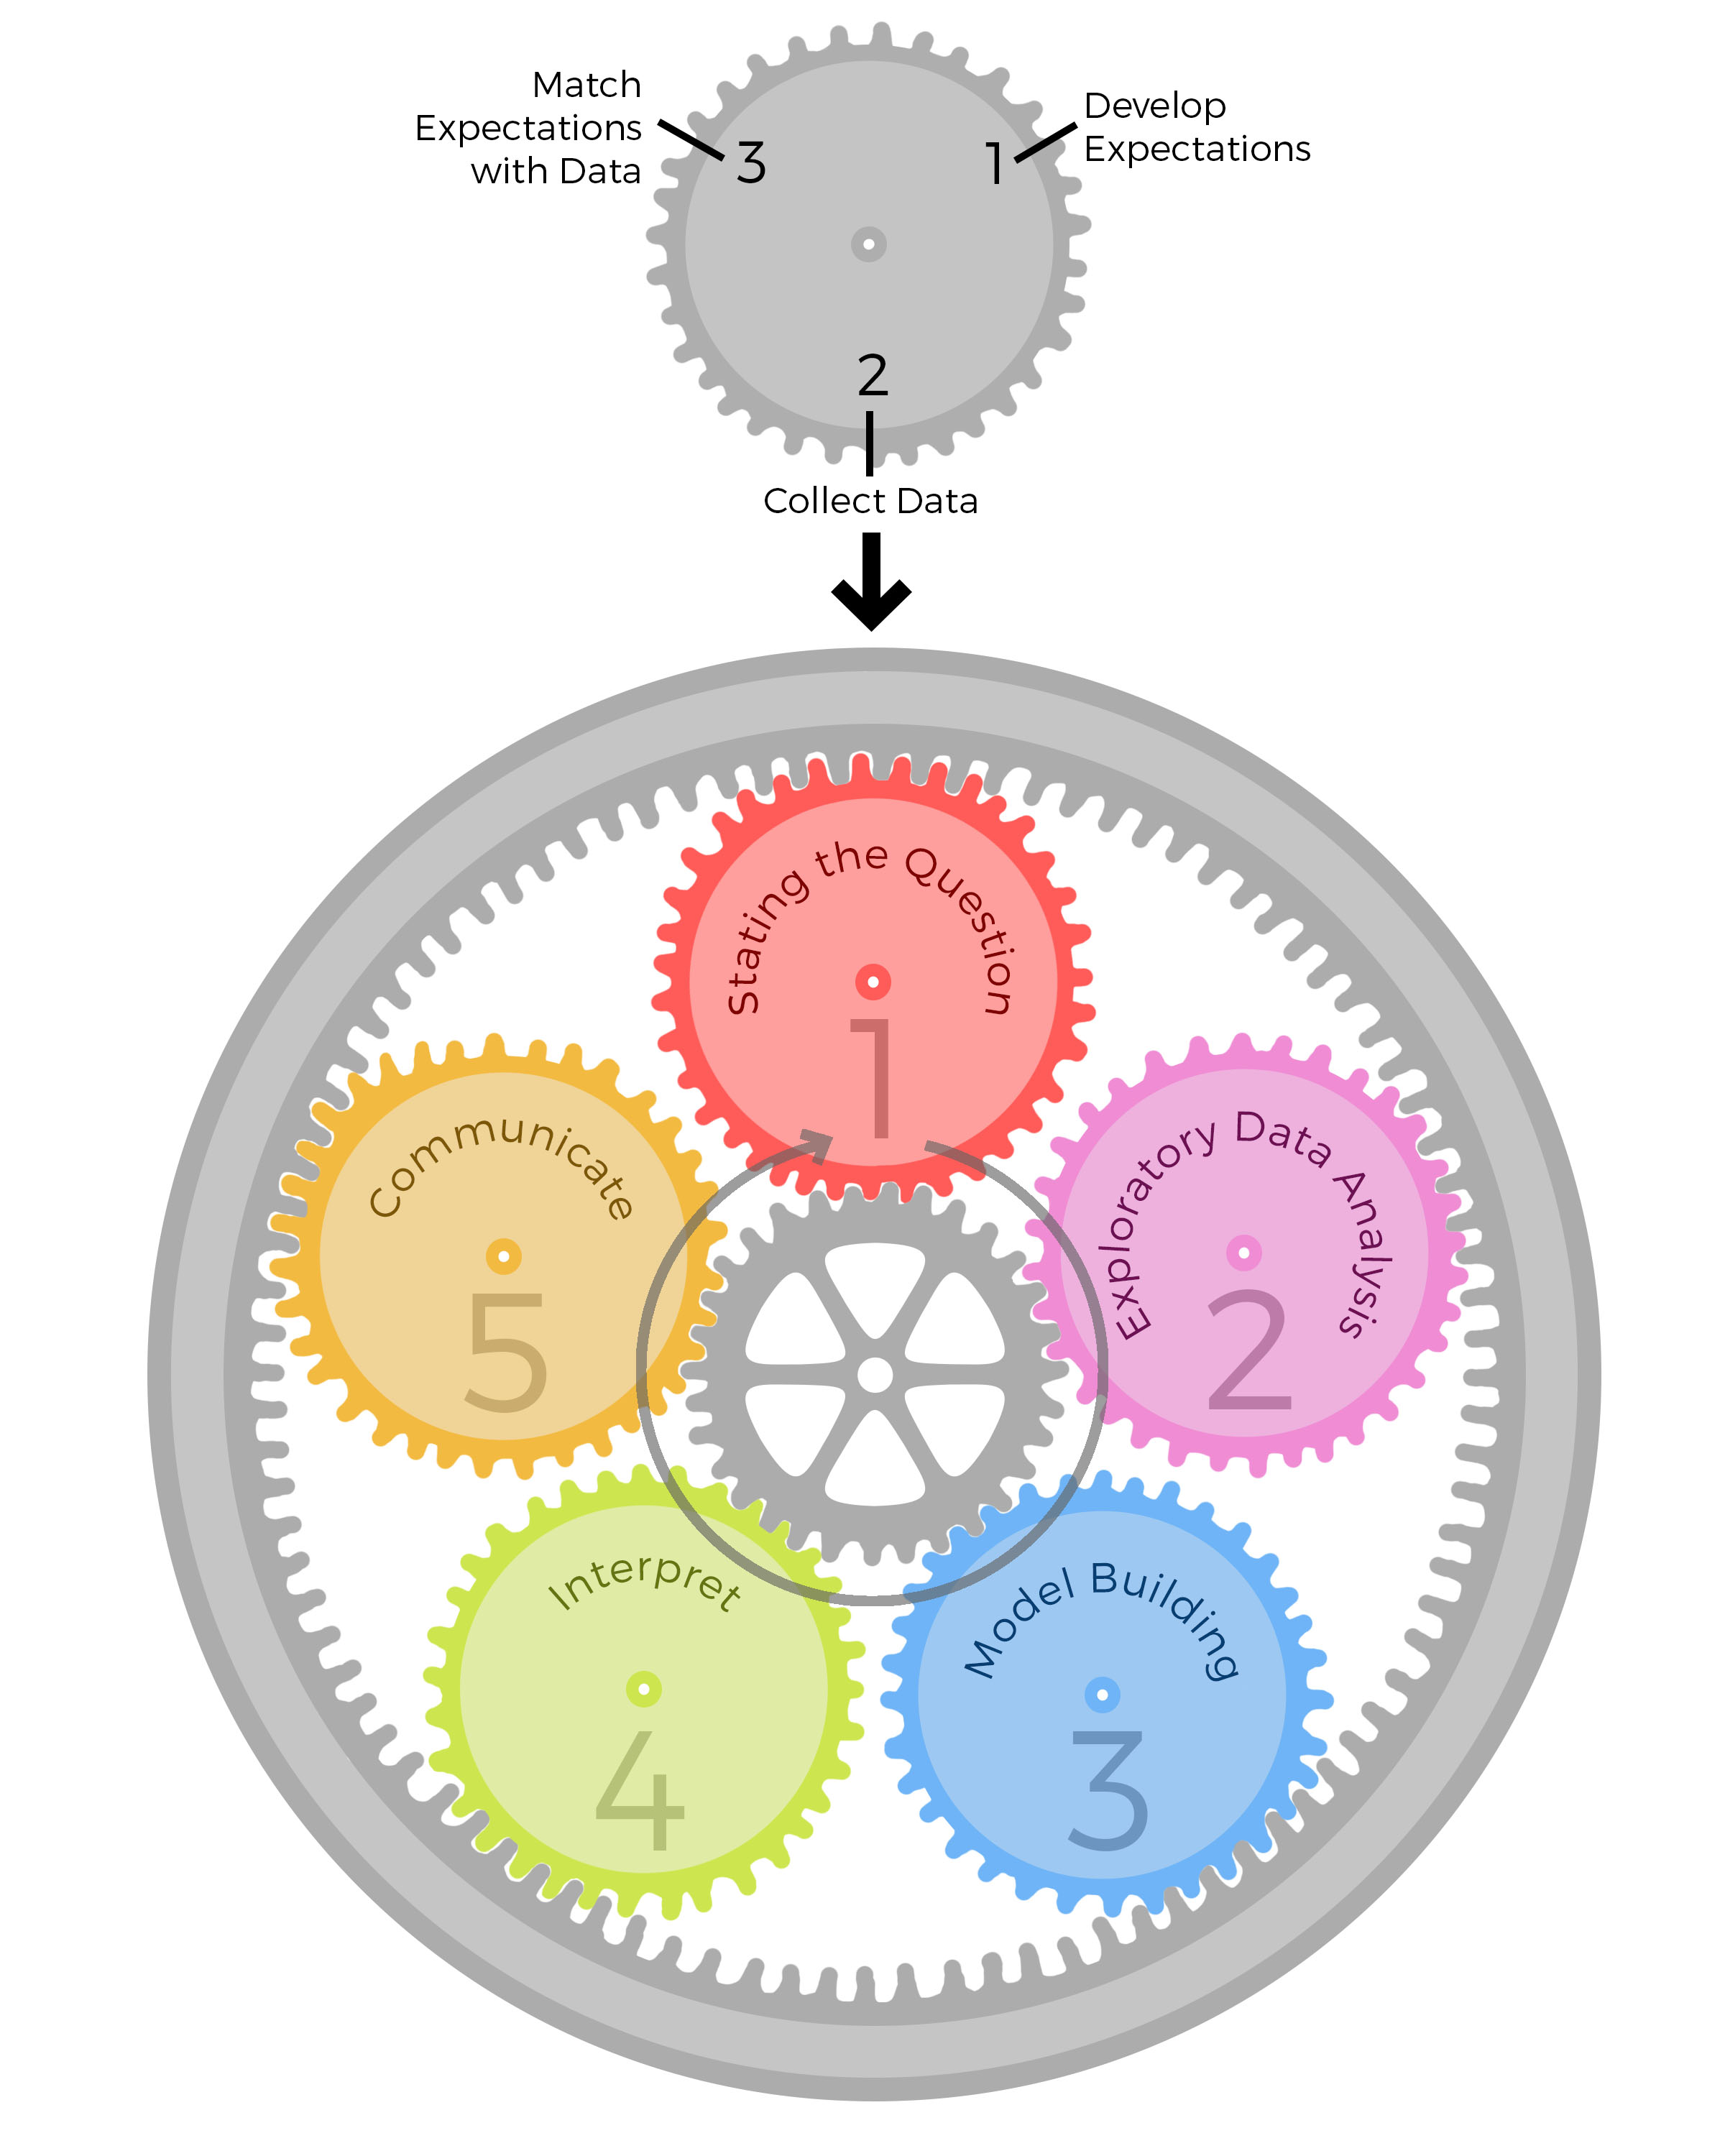
\includegraphics[width = 3in]{epicycle.png}
	\caption{Modelo de Epiciclos de Análisis de Datos (Fuente Peng y Matsui, 2017)}
\end{figure}

\subsection{Tareas Comunes en la Ciencia de Datos}
Hemos hablado de la ciencia de datos y su carácter predictivo. Las tareas mas comunes para lo cual se utiliza la ciencia de datos son las siguientes.

\begin{itemize}
	\item \textbf{Clasificación:} Decidir si algo pertenece a una categoría u otra. Harrington define la clasificación como la tarea de predecir a que tipo de clase pertenece una instancia (ejemplo) de la data propia de los métodos supervisados \cite{harrington}.
	\item \textbf{Puntuación:} Predecir o estimar un valor numérico, tal como lo es un precio o la probabilidad de un fenómeno. Alpaydin define esto como la extracción de reglas de los datos de los cuales se puede esperar estadísticamente un comportamiento similar y por lo cual se pueden efectuar predicciones correctas para instancias nuevas \cite{alpaydin}.
	\item \textbf{Ranking:} Aprender a ordenar objetos por preferencias
	\item \textbf{Agrupamientos:} Agrupar objetos en grupos de características homogéneas. Las técnicas de agrupamiento son típicas de los métodos de aprendizaje automatizado no-supervisados, donde en vez de buscar clasificar en clases conocidas o puntuar con valores ciertos, se busca la características comunes de la data para la agrupación de la misma en clases, tomando en cuenta que dichas clases no son conocidas a priori \cite{harrington}. 
	\item \textbf{Relaciones:} Encontrar relaciones o causas potenciales de efecto tal cual se ven en la data. Para Alpaydin la regresión lineal es un perfecto ejemplo de búsqueda de relaciones en la ciencia de datos, donde existe una función con un juego de parámetros asociados $y = g(x \mid \theta)$, $g(.)$ es el modelo y $\theta$ son sus parámetros. $Y$ es un número dentro de una regresión y $g(.)$ es la función de la regresión \cite{alpaydin}
	\item \textbf{Caracterizaciones:} Utilización general de visualizaciones y reportes de la data. Un ejemplo notable lo da Witten y Frank al referirse a la técnica de \emph{Market Basket Analysis} dentro de la mercadotecnia \cite{datamining}. En dicha técnica se busca que otros artículos comprarán los consumidores basados en el comportamiento registrado de sus compras pasadas. En términos matemáticos, estamos buscando $P(Y \mid X,D) = x_i$ donde $D$ es el juego conocido de datos históricos de los movimientos comerciales de los consumidores. 
\end{itemize}
